\documentclass{article}


% if you need to pass options to natbib, use, e.g.:
%     \PassOptionsToPackage{numbers, compress}{natbib}
% before loading neurips_2023


% ready for submission
\usepackage[final]{neurips_2023}


% to compile a preprint version, e.g., for submission to arXiv, add add the
% [preprint] option:
%     \usepackage[preprint]{neurips_2023}


% to compile a camera-ready version, add the [final] option, e.g.:
%     \usepackage[final]{neurips_2023}


% to avoid loading the natbib package, add option nonatbib:
%    \usepackage[nonatbib]{neurips_2023}


\usepackage[utf8]{inputenc} % allow utf-8 input
\usepackage[T1]{fontenc}    % use 8-bit T1 fonts
\usepackage{hyperref}       % hyperlinks
\usepackage{url}            % simple URL typesetting
\usepackage{booktabs}       % professional-quality tables
\usepackage{amsfonts}       % blackboard math symbols
\usepackage{nicefrac}       % compact symbols for 1/2, etc.
\usepackage{microtype}      % microtypography
\usepackage{xcolor}         % colors
\usepackage{graphicx}       % images
\graphicspath{ {./img/} }


\title{Proyecto Final Aprendizaje Automático}


% The \author macro works with any number of authors. There are two commands
% used to separate the names and addresses of multiple authors: \And and \AND.
%
% Using \And between authors leaves it to LaTeX to determine where to break the
% lines. Using \AND forces a line break at that point. So, if LaTeX puts 3 of 4
% authors names on the first line, and the last on the second line, try using
% \AND instead of \And before the third author name.


\author{%
    Lucía Herraiz Cano\\
    Aprendizaje Automático\\
    Universidad Pontificia Comillas\\
    Abril 2025\\
    \texttt{202300465@alu.comillas.edu} \\
}


\begin{document}


\maketitle


\begin{abstract}
  En este proyecto se desarrolla un análisis predictivo sobre el rendimiento 
  académico de estudiantes de secundaria en dos institutos de Madrid durante 
  el año 2005. A partir de un conjunto de datos, se construyen y comparan dos 
  modelos para predecir la nota final del curso (T3). También se lleva a cabo 
  un estudio de los datos y de las variables más influyentes en el desarrollo
  del estudiante. Este estudio busca no solo obtener predicciones precisas, 
  sino también generar conocimiento accionable para mejorar el rendimiento 
  estudiantil desde una perspectiva integral.
\end{abstract}


\section{Exploratory data analysis}


En esta sección se analiza la estructura y distribución del conjunto de datos, identificando patrones, valores atípicos y relaciones relevantes entre variables. También se detalla el proceso de limpieza y preparación necesario para el modelado posterior.


\subsection{Limpieza de datos}


El proceso de limpieza de datos viene recogido en la función \texttt{data\_cleaning\_pipeline}
e incluye el manejo de outliers, la imputación de valores faltantes, la corrección de errores, la codificación de las variables 
categóricas y la estandarización de los datos.

Sólo 5 variables tenían valores faltantes, y con el objetivo de perder la menor cantidad de datos, todos los valores se han imputado siguiendo distintas estrategias.
\textit{AlcSem, Relfam} y \textit{TiempoEstudio} han sido imputadas por la moda al ser variables categóricas, y tener menos de un 3\% de valores faltantes. \textit{Medu} y \textit{Pedu}, 
al tener un porcentaje más relevante de valores faltantes, tener una correlación alta (0.653), y al ser variables con mucho peso, como se verá posteriormente, han sido imputadas con un regresor (IterativeImputer) que emplea el resto de datos
para predecir sus valores de manera más robusta. 

Respecto a los outliers, la variable más llamativa fue \textit{faltas}. Se estableció un valor máximo de 150, correspondiente al número de días lectivos del calendario escolar estándar, considerando 
cualquier valor superior como erróneo. No se eliminaron registros, ya que \textit{faltas} mostró ser una variable altamente relevante.

% FOTO OUTLIERS ???? XXXXXXXXXXXXXXXXXXXXXXXXXXXXXX

Se han corregido los datos de la columna \textit{razon} al tener claves distintas para el mismo valor ("otras", "otros").

Finalmente, tras estudiar el balance de las clases, se ha visto que \textit{EstPadres, EstSup} y \textit{apoyo} están claramente desbalanceadas (80\%-20\%). Sin embargo, dado que ninguna es una variable
muy relevante, y dado que los resultados reflejan bien el balance que se suele dar en la población real, se ha decidido mantener los datos y tener cuidado con los modelos que le den relevancia a estas variables.

\subsection{Análisis no supervisado}


Con el objetivo de comprender mejor la relevancia y relación de las variables, se han implementado técnicas de aprendizaje no supervisado, que se pueden consultar en los ficheros \textit{Exploratory\_Data\_Analysis} y \textit{Model1\_Testing}.

En primer lugar, se ha implementado \textbf{Principal Component Analysis (PCA)} con el objetivo de ver si la reducicción de la dimensionalidad aporta beneficios y para ver los componentes principales. 
La varianza explicada con 2 y 3 componentes principales es menor al 30\%, sin embargo, el estudio de sus loadings aporta información relevante. Para el 1º modelo, como cabía esperar, las variables
más relevantes son \textit{T1, T2} y \textit{suspensos}, pero es más interesante estudiar el 2º modelo, puesto que al eliminar estas variables, las sutituyen \textit{AlcSem, AlcFin, SalAm, TiempoLib} y otras, que
 indican que después de las \textbf{notas}, la \textbf{vida social del estudiante} es uno de los factores más relevantes para su desempeño. Además de estos, un tercer grupo de variables de peso que aparecen en los PC son \textit{Medu, Pedu, Relfam} y empleando \textbf{Recursive Feature Elimination (RFE)} 
se obtiene también \textit{Mtrab\_docencia} y \textit{Ptrab\_docencia}, lo que indica que el \textbf{entorno familiar} es otro de los factores más influyentes en las notas. 

\begin{figure}[h!]
  \centering
  \begin{minipage}[b]{0.45\textwidth}
      \centering
      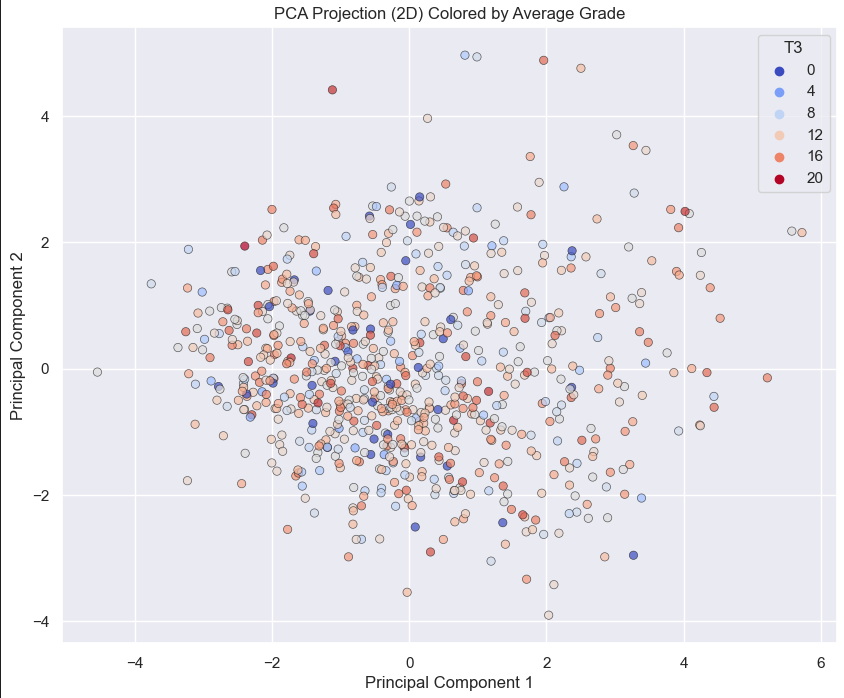
\includegraphics[scale=0.30]{PCA2PC.png}
      \caption*{(a) PCA con 2 componentes principales}
  \end{minipage}
  \hfill
  \begin{minipage}[b]{0.45\textwidth}
      \centering
      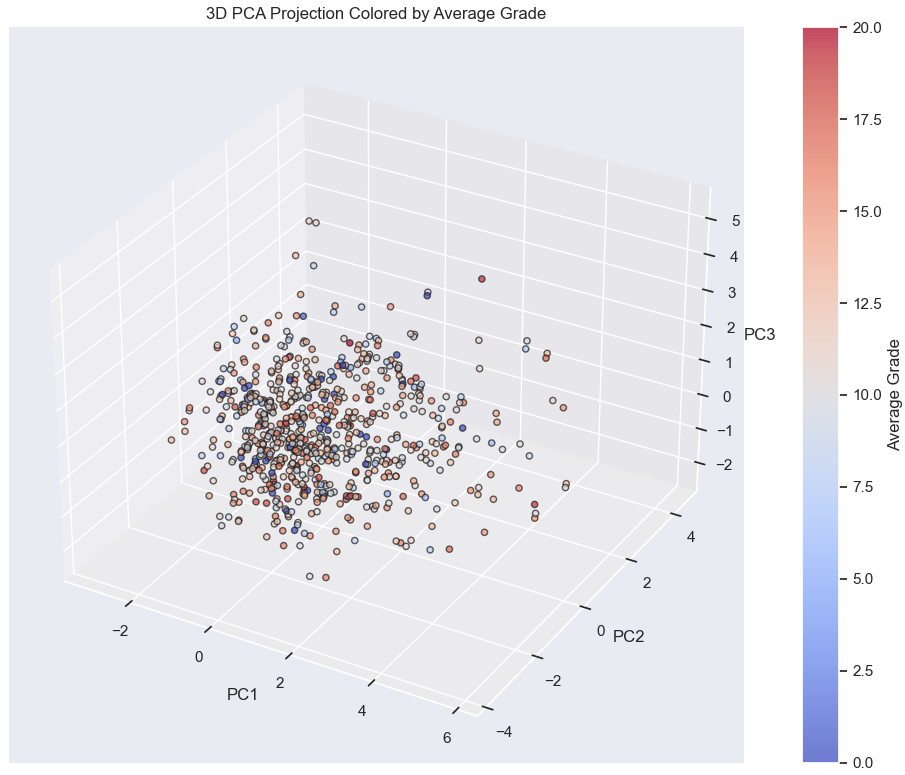
\includegraphics[scale=0.28]{PCA3PC.png}
      \caption*{(b) PCA con 3 componentes principales}
  \end{minipage}
  \caption{Visualización de los datos proyectados sobre 2 y 3 componentes principales mediante PCA.}
\end{figure}


Sin embargo, PCA requiere 16 componentes para explicar el 80\% de la varianza. Al combinarlo con modelos como SVR o regresión lineal, su rendimiento disminuyó, por lo que se descartó su uso 
más allá de la exploración inicial. Este comportamiento podría deberse a la naturaleza lineal de PCA, incapaz de capturar relaciones no lineales en los datos. Por ello, se probaron 
técnicas no lineales como \textbf{ISOMAP} y \textbf{Kernel-PCA}, que operan en espacios transformados mediante distancias geodésicas o kernels y que pueden capturar relaciones más complejas entre los datos. No obstante, su combinación con modelos predictivos redujo el rendimiento entre un 20-30\%. 
Podemos conluir que la reducción de dimensionalidad implica pérdida de información relevante para la predicción. Las variables no son fácilmente separables.

Asimismo, se aplicaron técnicas de \textbf{Clustering} a los datos (combinadas con PCA). Utilizando la métrica del \textit{Elbow Method} y de la \textit{Silueta}, el número óptimo de clusters  se sitúa entre 2 y 3, en línea con los grupos de variables relevantes identificados anteriormente. No obstante, los valores obtenidos tras aplicar K-Means (Silueta: 0.233; Índice de Davies-Bouldin: 1.341) indican una calidad media en la segmentación, reafirmando la dificultad al separar los datos. 
Experimentalmente, se probó a añadir una nueva variable indicando la pertenecia a los clusters de los datos para entrenar a un regresor lineal, pero esto no modificó su \textit{performance}, por lo que finalmente, usando la filosofía de la \textit{Navaja de Occam},
se descartó el uso activo del clustering en los modelos.

\begin{figure}[h!]
  \centering
  \begin{minipage}[b]{0.45\textwidth}
      \centering
      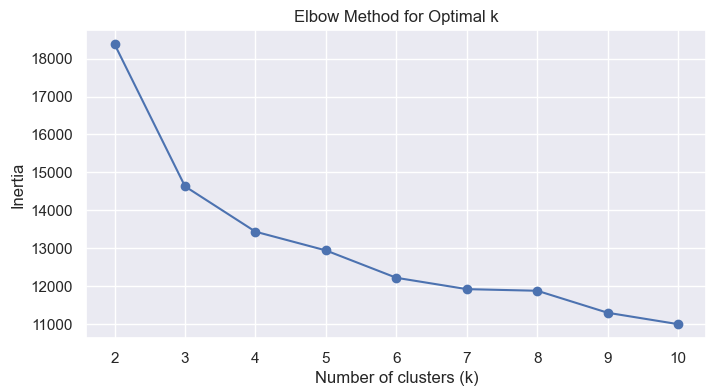
\includegraphics[scale=0.40]{Elbow_Method.png}
      \caption*{(a) Elbow Method}
  \end{minipage}
  \hfill
  \begin{minipage}[b]{0.45\textwidth}
      \centering
      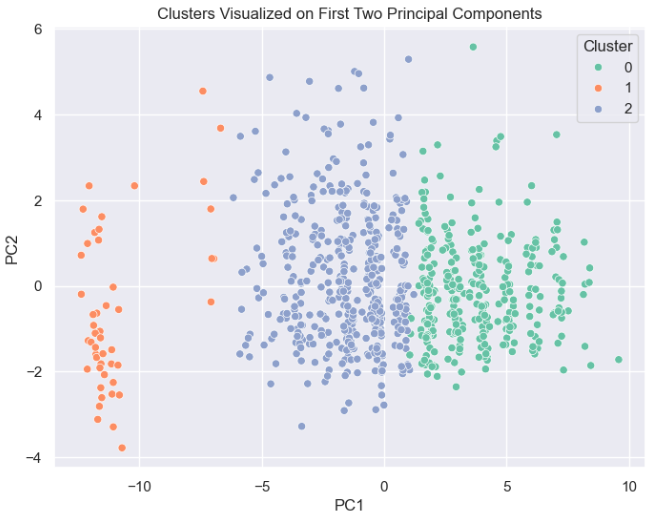
\includegraphics[scale=0.4]{Clusters.png}
      \caption*{(b) Clusters}
  \end{minipage}
  \caption{Análisis por clustering}
\end{figure}

\subsection{Análisis adicional}


A modo de comprobación del análisis anterior, y con el objetivo de descubrir nuevos patrones, se han empleado las características de varios modelos para ver la relevancia de las variables.

Se ha estudiado la representación conjunta de cada par de variables, empleando como código de color las distintas clases para identificar posibles relaciones\footnote{Ver la matriz completa en el fichero \textit{Exploratory\_Data\_Analysis}}, pero sólo se ha encontrado un patrón claro con \textit{T1} y \textit{T2}.

\begin{figure}[ht]
  \centering
  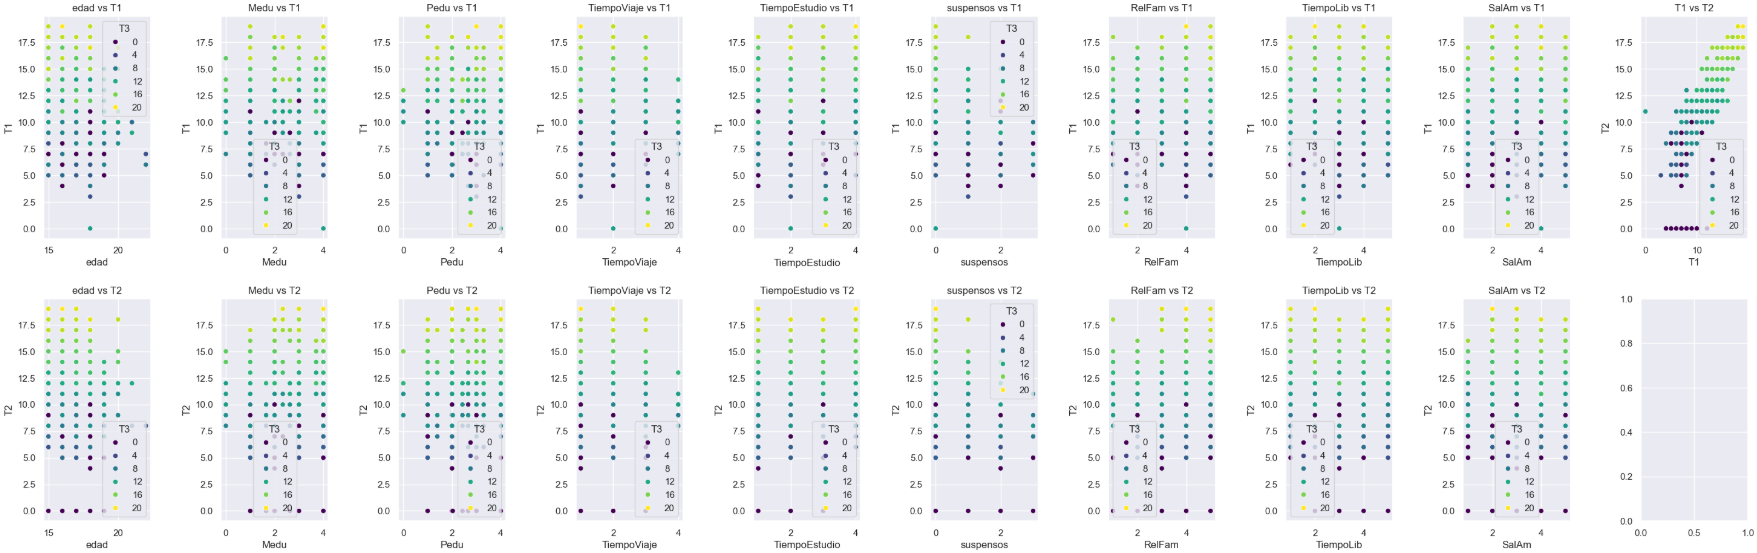
\includegraphics[width=0.9\textwidth]{Plot_Var_T1T2.png}
  \caption{Scatter Plot con T1 y T2}\label{fig:scatter}
\end{figure}

Uno de los algoritmos con mejor desempeño en ambos modelos, como se verá más adelante, es \textbf{Random Forest}. Vemos que las variables que considera más importantes coinciden con las obtenidas con PCA en ambos casos.


\begin{figure}[ht]
  \centering
  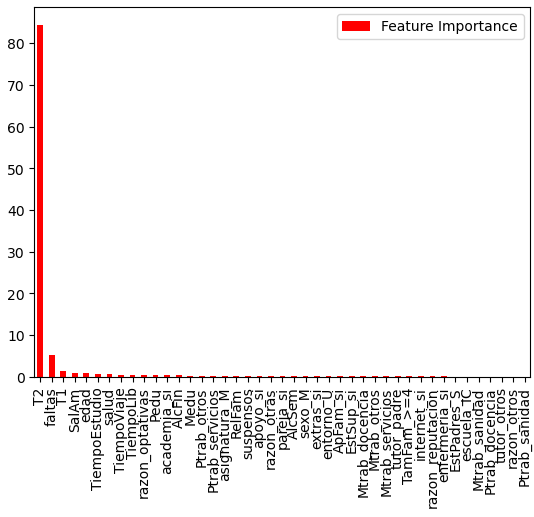
\includegraphics[width=0.4\textwidth]{RF_var.png}
  \caption{Feature importance en Random Forest}\label{fig:t1t2}
\end{figure}

A pesar de que el modelo de \textbf{regresión} logística no tiene el mejor rendimiento, al ser un clasificador, es interesante emplearlo, junto con regularización Lasso, para ver la evolución de los pesos de las variables para cada una de las clases, lo que aporta una mayor profundidad en el análisis.
El estudio se ha realizado sin tener en cuante \textit{T1} y \textit{T2} y podemos ver que para las notas más bajas las variables relacionadas con la vida social y la familia son las más importantes, mientras que para las notas más altas, influyen variables más generales.

\begin{figure}[h!]
  \centering
  \begin{minipage}[b]{0.3\textwidth}
      \centering
      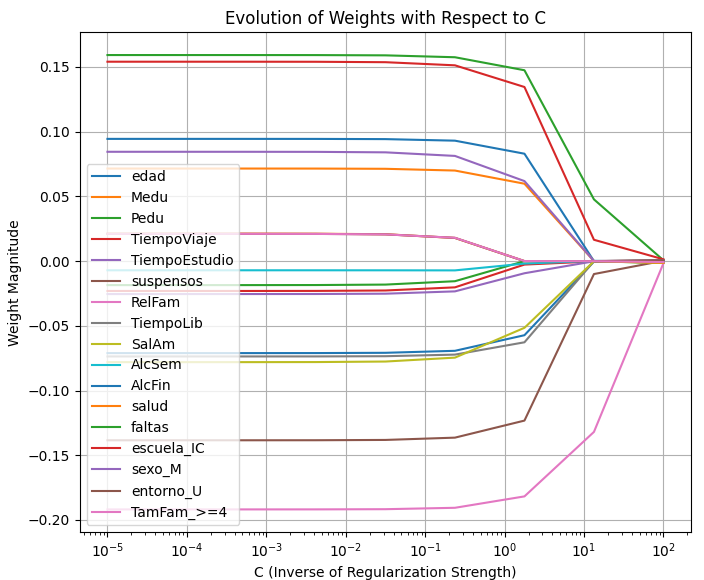
\includegraphics[scale=0.3]{FI_Class1.png}
      \caption*{(a) Clase 1}
  \end{minipage}
  \hfill
  \begin{minipage}[b]{0.3\textwidth}
      \centering
      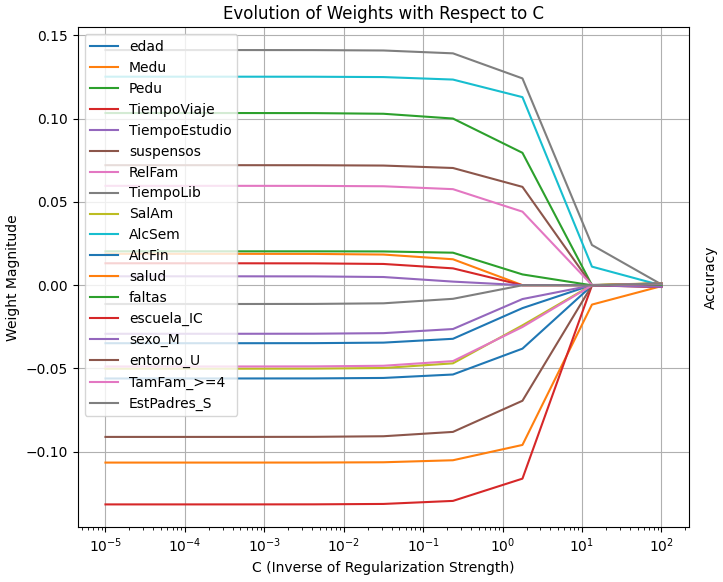
\includegraphics[scale=0.3]{FI_Class10.png}
      \caption*{(b) Clase 10}
  \end{minipage}
  \hfill
  \begin{minipage}[b]{0.3\textwidth}
      \centering
      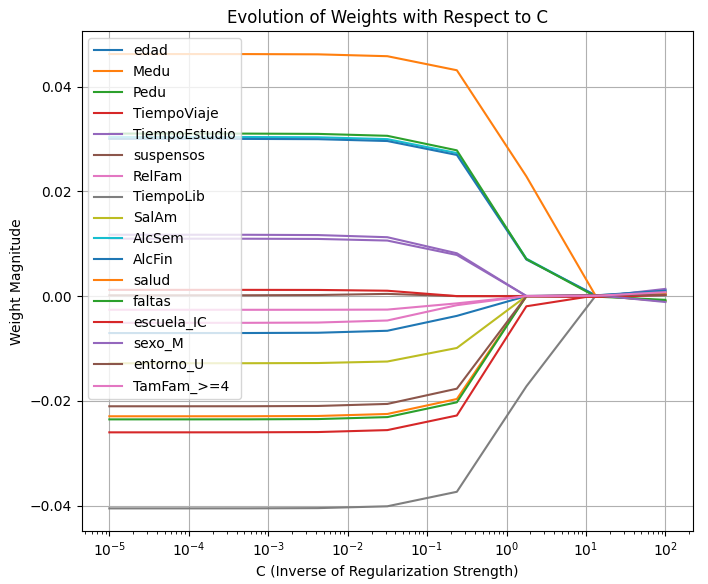
\includegraphics[scale=0.3]{FI_Class20.png}
      \caption*{(c) Clase 20}
  \end{minipage}
  \caption{Feature Importance para tres clases}
\end{figure}


\section{Implementación y comparación de los dos modelos predictivos}

En esta sección se presentan los algoritmos con mayor rendimiento para ambos enfoques, junto con los criterios que justifican la elección de los modelos finales.

\subsection{Modelo 1: Enfoque Predictivo con la Información Completa del Dataset}

Tras analizar múltiples modelos, se concluyó que los regresores superan consistentemente a los clasificadores, con una mejora media del 20\% en las métricas. Por ello, se descartó en una fase inicial continuar con clasificadores y se priorizó profundizar en modelos de regresión.

Los modelos de clasificación probados junto con su \textit{Accuracy} media fueron \textbf{Logistic Regression} (0.28), \textbf{Logistic Regression con Kernel-PCA} (0.57), \textbf{Support Vector Classifier (SVC)} (0.31), \textbf{Random Forest Classifier} (0.46) y  \textbf{Bagging Classifier} (0.45).\footnote{La implementación de estos modelos y otras métricas se pueden consultar en \textit{Model1\_Testing}}

La Tabla~\ref{sample-table} muestra los mejores modelos de regresión. Para garantizar la consistencia de las métricas, los valores presentados corresponden a los promedios obtenidos tras entrenar 300 modelos por cada técnica, utilizando datos mezclados en cada iteración.

Otros modelos de regresión probados, junto con sus valores \textit{$R^2$} medios fueron \textbf{Bagging Regressor} (0.80), \textbf{Support Vector Regressor (SVR) con Kernel-PCA} (0.80), \textbf{Linear Regression con ISOMAP} (0.61) y \textbf{Linear Regression con Kernel-PCA} (0.80).

\begin{table}
  \caption{Modelos de regresión}
  \label{sample-table}
  \centering
  \begin{tabular}{lcccc}
    \toprule
    \multicolumn{5}{c}{Comparativa entre modelos} \\
    \cmidrule(r){1-5}
    Nombre & R² Score Test & MAE & MSE & R² Score Train \\
    \midrule
    Linear Regression & 0.8301 $\pm$ 0.033 & 0.2513 & 0.1693 & 0.853 \\
    LR con relaciones & 0.8338 $\pm$ 0.0319 & 0.2496 & 0.1682 & 0.855 \\
    Ensemble de LR    & 0.8332 $\pm$ 0.0339 & 0.2491 & 0.1669 & 0.852 \\
    Stack             & 0.8332 $\pm$ 0.0339 & 0.2513 & 0.1693 & 0.853 \\
    Bagging           & 0.830  $\pm$ 0.033  & 0.2513 & 0.1693 & 0.853 \\
    Random Forest     & 0.830  $\pm$ 0.033  & 0.2513 & 0.1693 & 0.853 \\
    SVR               & 0.830  $\pm$ 0.033  & 0.2513 & 0.1693 & 0.853 \\
    \bottomrule
  \end{tabular}
\end{table}

\subsection{Modelo 2: Enfoque Predictivo sin las variables T1 y T2}

Al eliminar las variables de más peso, los modelos reducen a la mitad su poder predictivo.

\section{Conclusiones accionables}

El análisis de los datos nos indica que influyen tres grupos principales de variables a la hora de predecir el desempeño de los estudientes, las \textbf{notas previas}, la \textbf{vida social} del estudiante, y su \textbf{entorno familiar}.
Con esta información, los centros educativos pueden enfocar sus medidas en estas áreas. Sensibilizar al alumnado sobre la importancia de equilibrar vida social y estudio puede favorecer su rendimiento. Asimismo, promover políticas de 
conciliación familiar podría tener un impacto positivo en sus resultados académicos.

The only supported style file for NeurIPS 2023 is \verb+neurips_2023.sty+,
rewritten for \LaTeXe{}.  \textbf{Previous style files for \LaTeX{} 2.09,
  Microsoft Word, and RTF are no longer supported!}


The \LaTeX{} style file contains three optional arguments: \verb+final+, which
creates a camera-ready copy, \verb+preprint+, which creates a preprint for
submission to, e.g., arXiv, and \verb+nonatbib+, which will not load the
\verb+natbib+ package for you in case of package clash.


\paragraph{Preprint option}
If you wish to post a preprint of your work online, e.g., on arXiv, using the
NeurIPS style, please use the \verb+preprint+ option. This will create a
nonanonymized version of your work with the text ``Preprint. Work in progress.''
in the footer. This version may be distributed as you see fit, as long as you do not say which conference it was submitted to. Please \textbf{do
  not} use the \verb+final+ option, which should \textbf{only} be used for
papers accepted to NeurIPS. 


At submission time, please omit the \verb+final+ and \verb+preprint+
options. This will anonymize your submission and add line numbers to aid
review. Please do \emph{not} refer to these line numbers in your paper as they
will be removed during generation of camera-ready copies.


The file \verb+neurips_2023.tex+ may be used as a ``shell'' for writing your
paper. All you have to do is replace the author, title, abstract, and text of
the paper with your own.



\section{General formatting instructions}
\label{gen_inst}


The text must be confined within a rectangle 5.5~inches (33~picas) wide and
9~inches (54~picas) long. The left margin is 1.5~inch (9~picas).  Use 10~point
type with a vertical spacing (leading) of 11~points.  Times New Roman is the
preferred typeface throughout, and will be selected for you by default.
Paragraphs are separated by \nicefrac{1}{2}~line space (5.5 points), with no
indentation.


The paper title should be 17~point, initial caps/lower case, bold, centered
between two horizontal rules. The top rule should be 4~points thick and the
bottom rule should be 1~point thick. Allow \nicefrac{1}{4}~inch space above and
below the title to rules. All pages should start at 1~inch (6~picas) from the
top of the page.


For the final version, authors' names are set in boldface, and each name is
centered above the corresponding address. The lead author's name is to be listed
first (left-most), and the co-authors' names (if different address) are set to
follow. If there is only one co-author, list both author and co-author side by
side.


Please pay special attention to the instructions in Section 
regarding figures, tables, acknowledgments, and references.


\section{Headings: first level}
\label{headings}


All headings should be lower case (except for first word and proper nouns),
flush left, and bold.


First-level headings should be in 12-point type.


\subsection{Headings: second level}


Second-level headings should be in 10-point type.


\subsubsection{Headings: third level}


Third-level headings should be in 10-point type.


\paragraph{Paragraphs}


There is also a \verb+\paragraph+ command available, which sets the heading in
bold, flush left, and inline with the text, with the heading followed by 1\,em
of space.


\section{Citations, figures, tables, references}
\label{others}


These instructions apply to everyone.


\subsection{Citations within the text}


The \verb+natbib+ package will be loaded for you by default.  Citations may be
author/year or numeric, as long as you maintain internal consistency.  As to the
format of the references themselves, any style is acceptable as long as it is
used consistently.


The documentation for \verb+natbib+ may be found at
\begin{center}
  \url{http://mirrors.ctan.org/macros/latex/contrib/natbib/natnotes.pdf}
\end{center}
Of note is the command \verb+\citet+, which produces citations appropriate for
use in inline text.  For example,
\begin{verbatim}
   \citet{hasselmo} investigated\dots
\end{verbatim}
produces
\begin{quote}
  Hasselmo, et al.\ (1995) investigated\dots
\end{quote}


If you wish to load the \verb+natbib+ package with options, you may add the
following before loading the \verb+neurips_2023+ package:
\begin{verbatim}
   \PassOptionsToPackage{options}{natbib}
\end{verbatim}


If \verb+natbib+ clashes with another package you load, you can add the optional
argument \verb+nonatbib+ when loading the style file:
\begin{verbatim}
   \usepackage[nonatbib]{neurips_2023}
\end{verbatim}


As submission is double blind, refer to your own published work in the third
person. That is, use ``In the previous work of Jones et al.\ [4],'' not ``In our
previous work [4].'' If you cite your other papers that are not widely available
(e.g., a journal paper under review), use anonymous author names in the
citation, e.g., an author of the form ``A.\ Anonymous'' and include a copy of the anonymized paper in the supplementary material.


\subsection{Footnotes}


Footnotes should be used sparingly.  If you do require a footnote, indicate
footnotes with a number\footnote{Sample of the first footnote.} in the
text. Place the footnotes at the bottom of the page on which they appear.
Precede the footnote with a horizontal rule of 2~inches (12~picas).


Note that footnotes are properly typeset \emph{after} punctuation
marks.\footnote{As in this example.}


\subsection{Figures}


\begin{figure}
  \centering
  \fbox{\rule[-.5cm]{0cm}{4cm} \rule[-.5cm]{4cm}{0cm}}
  \caption{Sample figure caption.}
\end{figure}


All artwork must be neat, clean, and legible. Lines should be dark enough for
purposes of reproduction. The figure number and caption always appear after the
figure. Place one line space before the figure caption and one line space after
the figure. The figure caption should be lower case (except for first word and
proper nouns); figures are numbered consecutively.


You may use color figures.  However, it is best for the figure captions and the
paper body to be legible if the paper is printed in either black/white or in
color.


\subsection{Tables}


All tables must be centered, neat, clean and legible.  The table number and
%title always appear before the table.  See Table~\ref{sample-table}.


Place one line space before the table title, one line space after the
table title, and one line space after the table. The table title must
be lower case (except for first word and proper nouns); tables are
numbered consecutively.


Note that publication-quality tables \emph{do not contain vertical rules.} We
strongly suggest the use of the \verb+booktabs+ package, which allows for
typesetting high-quality, professional tables:
\begin{center}
  \url{https://www.ctan.org/pkg/booktabs}
\end{center}
%This package was used to typeset Table~\ref{sample-table}.



\subsection{Math}
%Note that display math in bare TeX commands will not create correct line numbers for submission. Please use LaTeX (or AMSTeX) commands for unnumbered display math. (You really shouldn't be using \$\$ anyway; see \url{https://tex.stackexchange.com/questions/503/why-is-preferable-to} and \url{https://tex.stackexchange.com/questions/40492/what-are-the-differences-between-align-equation-and-displaymath} for more information.)

\subsection{Final instructions}

Do not change any aspects of the formatting parameters in the style files.  In
particular, do not modify the width or length of the rectangle the text should
fit into, and do not change font sizes (except perhaps in the
\textbf{References} section; see below). Please note that pages should be
numbered.


\section{Preparing PDF files}


Please prepare submission files with paper size ``US Letter,'' and not, for
example, ``A4.''


Fonts were the main cause of problems in the past years. Your PDF file must only
contain Type 1 or Embedded TrueType fonts. Here are a few instructions to
achieve this.


\begin{itemize}


\item You should directly generate PDF files using \verb+pdflatex+.


\item You can check which fonts a PDF files uses.  In Acrobat Reader, select the
  menu Files$>$Document Properties$>$Fonts and select Show All Fonts. You can
  also use the program \verb+pdffonts+ which comes with \verb+xpdf+ and is
  available out-of-the-box on most Linux machines.


\item \verb+xfig+ "patterned" shapes are implemented with bitmap fonts.  Use
  "solid" shapes instead.


\item The \verb+\bbold+ package almost always uses bitmap fonts.  You should use
  the equivalent AMS Fonts:
\begin{verbatim}
   \usepackage{amsfonts}
\end{verbatim}
followed by, e.g., \verb+\mathbb{R}+, \verb+\mathbb{N}+, or \verb+\mathbb{C}+
for $\mathbb{R}$, $\mathbb{N}$ or $\mathbb{C}$.  You can also use the following
workaround for reals, natural and complex:
\begin{verbatim}
   \newcommand{\RR}{I\!\!R} %real numbers
   \newcommand{\Nat}{I\!\!N} %natural numbers
   \newcommand{\CC}{I\!\!\!\!C} %complex numbers
\end{verbatim}
Note that \verb+amsfonts+ is automatically loaded by the \verb+amssymb+ package.


\end{itemize}


If your file contains type 3 fonts or non embedded TrueType fonts, we will ask
you to fix it.


\subsection{Margins in \LaTeX{}}


Most of the margin problems come from figures positioned by hand using
\verb+\special+ or other commands. We suggest using the command
\verb+\includegraphics+ from the \verb+graphicx+ package. Always specify the
figure width as a multiple of the line width as in the example below:
\begin{verbatim}
   \usepackage[pdftex]{graphicx} ...
   \includegraphics[width=0.8\linewidth]{myfile.pdf}
\end{verbatim}
See Section 4.4 in the graphics bundle documentation
(\url{http://mirrors.ctan.org/macros/latex/required/graphics/grfguide.pdf})


A number of width problems arise when \LaTeX{} cannot properly hyphenate a
line. Please give LaTeX hyphenation hints using the \verb+\-+ command when
necessary.


\begin{ack}
Use unnumbered first level headings for the acknowledgments. All acknowledgments
go at the end of the paper before the list of references. Moreover, you are required to declare
funding (financial activities supporting the submitted work) and competing interests (related financial activities outside the submitted work).
More information about this disclosure can be found at: \url{https://neurips.cc/Conferences/2023/PaperInformation/FundingDisclosure}.


Do {\bf not} include this section in the anonymized submission, only in the final paper. You can use the \texttt{ack} environment provided in the style file to autmoatically hide this section in the anonymized submission.
\end{ack}



\section{Supplementary Material}

Authors may wish to optionally include extra information (complete proofs, additional experiments and plots) in the appendix. All such materials should be part of the supplemental material (submitted separately) and should NOT be included in the main submission.


\section*{References}


References follow the acknowledgments in the camera-ready paper. Use unnumbered first-level heading for
the references. Any choice of citation style is acceptable as long as you are
consistent. It is permissible to reduce the font size to \verb+small+ (9 point)
when listing the references.
Note that the Reference section does not count towards the page limit.
\medskip


{
\small


[1] Alexander, J.A.\ \& Mozer, M.C.\ (1995) Template-based algorithms for
connectionist rule extraction. In G.\ Tesauro, D.S.\ Touretzky and T.K.\ Leen
(eds.), {\it Advances in Neural Information Processing Systems 7},
pp.\ 609--616. Cambridge, MA: MIT Press.


[2] Bower, J.M.\ \& Beeman, D.\ (1995) {\it The Book of GENESIS: Exploring
  Realistic Neural Models with the GEneral NEural SImulation System.}  New York:
TELOS/Springer--Verlag.


[3] Hasselmo, M.E., Schnell, E.\ \& Barkai, E.\ (1995) Dynamics of learning and
recall at excitatory recurrent synapses and cholinergic modulation in rat
hippocampal region CA3. {\it Journal of Neuroscience} {\bf 15}(7):5249-5262.
}

%%%%%%%%%%%%%%%%%%%%%%%%%%%%%%%%%%%%%%%%%%%%%%%%%%%%%%%%%%%%


\end{document}